\subsection{Fast Diagonalization Method (FDM)}
    \BA{NEPTUNE interested in high-order methods- why?:
    \begin{itemize}
        \item  Better approximation properties (provided sufficient regularity- N.B. \emph{Not} necessarily the case with funky BCs in a tokamak, but \emph{should} be fine in my case if I pick a nice model with nice BCs on a nice domain).
        \item  Better numerical approximation properties. (Recall that diagram from the NEPTUNE workshop with the traveling bump).
        \item  Better suited to modern computer architectures. (Ask Pablo for more clarification here.)
    \end{itemize}
    Why not?:
    \begin{itemize}
        \item  Massively worse computational complexity- very dense matrices, unless we find some way to mitigate this...
    \end{itemize}}

    \BA{These equations require more orthogonality than traditional FDM can offer, right? Right. However, here's the big idea: Why do we need to stick to a polynomial basis?  \\
    What I mean by that is this: When working with FDM, we're working with tensors product finite elements, ultimately constructed from finite elements on the interval. For the complexes with which we're familiar, these interval FEs use function spaces of polynomials $\calP_{p}$. Standard FDM constructs $\sim p$ interior basis functions $(\phi_{i})$ for $\calP_{p}$ (or at least $\calP_{p}$ with appropriate $0$ BCs) as $\phi_{i} \in \calP_{p}$, such that we have agency over $\sim p^{2}$ coefficients for the basis. One ``set'' of orthogonality relations requires $\sim \frac{1}{2}p^{2}$ conditions on the basis coefficients. Working in this way therefore, standard FDM can only achieve 2 sets of orthogonality relations, usually:
    \begin{align}
        \langle\phi_{i}, \phi_{j}\rangle  =  \delta_{i, j}  &&
        \langle\phi_{i}', \phi_{j}'\rangle  =  \lambda_{i}\delta_{i, j}
    \end{align}
    Taking a step back, however, we can ask ourselves: \emph{``Why must we choose the function space on the interval element to be $\calP_{p}$?''}.  \\
    If, say, we were looking for $\sim p$ \emph{independent} functions $(\phi_{i})$ in $\calP_{\frac{3}{2}p}$, then we have agency over $\sim \frac{3}{2}p^{2}$ coefficients, and thus can choose over basis to satisfy 3 sets of orthogonality relations, say:
    \begin{align}
        \langle\phi_{i}, \phi_{j}\rangle  =  \delta_{i, j}  &&
        \langle\phi_{i}', \phi_{j}'\rangle  =  \lambda_{i}\delta_{i, j}  &&
        \langle\phi_{i}'', \phi_{j}''\rangle  =  \mu_{i}\delta_{i, j}
    \end{align}
    As such, we would be constructing our complex from a complex on the interval:
    \begin{center}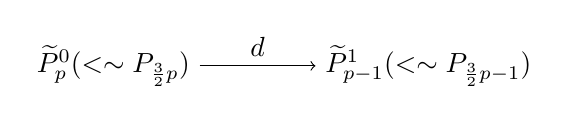
\begin{tikzpicture}[align = center, node distance = 4cm, auto]
        \node (0) at (0, 0) {$\widetilde{P}_{p}^{0}  (<  \sim  P_{\frac{3}{2}p})$};
        \node (1) at (4, 0) {$\widetilde{P}_{p - 1}^{1}  (<  \sim P_{\frac{3}{2}p - 1})$};        
        \draw[->] (0) -- (1)
            node[midway, above] {$d$};
    \end{tikzpicture}\end{center}
    These are exactly the orthogonality relations we would need to apply FDM to Stokes.}

    \BA{What about if we construct each basis function iteratively instead? Twice the max polynomial degree, but can all be computed in advance and just read from a database, and much more intuitive if we start playing with messy non-linear PDEs.}

    \BA{If we want to apply FDM to \emph{Navier--}Stokes, then we would want the following to be as infrequently non-zero as possible:
    \begin{align*}
        \langle\phi_{i}, \phi_{j}, \phi_{k}\rangle  &&
        \langle\phi_{i}', \phi_{j}, \phi_{k}\rangle  &&
        \langle\phi_{i}'', \phi_{j}', \phi_{k}\rangle
    \end{align*}
    as well as the following, which inherits its sparsity from that of $\langle\phi_{i}'', \phi_{j}', \phi_{k}\rangle$.
    \begin{equation*}
        \langle\phi_{i}', \phi_{j}', \phi_{k}'\rangle  =  - (\langle\phi_{i}'', \phi_{j}', \phi_{k}\rangle + \langle\phi_{i}', \phi_{j}'', \phi_{k}\rangle)
    \end{equation*}
    Unfortunately, this is not as simple as the sparsity for the linear case. I am not sure when different combinations of these can be enforced. If, say, we were going through the bases and adding the lowest-order polynomial for each basis function that can give nice sparsity, then we fail on $\phi_{2}$. Presuming $\phi_{1}  =  {\rm const}(1 - x^{2})^{2{\rm const}}$, we have $\phi_{1}  \geq  0$, thus making the condition $\langle\phi_{2}, \phi_{2}, \phi_{1}\rangle  =  0$ impossible.  \\
    This might not be a problem if we try and define all $(\phi_{i})$ concurrently, but I am really not sure how many $0$ values you'd be able to reach if that was the plan. You could just generally try to minimise the number of $0$ entries in the the $\sfA  :=  (\langle\phi_{i}, \phi_{j}, \phi_{k}\rangle)$, $\sfB  := (\langle\phi_{i}', \phi_{j}, \phi_{k}\rangle)$, $\sfC  :=  (\langle\phi_{i}'', \phi_{j}', \phi_{k}\rangle)$ tensors by---say---minimising $\|\sfA\|_{r}$, $\|\sfB\|_{r}$, $\|\sfC\|_{r}$ and taking $r \rightarrow  0$. There's also the question though of what the best sparsity pattern for these tensors would be to make each Krylov iterate as computationally efficient as possible, which, if we can't achieve optimal sparsity, might be something else specific.}
    